\chapter{Návrh}
Před samotnou implementací je třeba vyhotovit návrh systému. Behaviorální modely systému byly představeny již v kapitole \ref{chap:specification} Analýza požadavků. Nyní je třeba systém navrhnout ze strukturálního pohledu. Součástí návrhu je dekompozice problému na jednotlivé služby, návrh architektur jednotlivých služeb a~identifikace klíčových komponent. Návrh vychází z~podkladů, které byly vytvořeny v~kapitole \ref{chap:specification} Analýza požadavků. Tvorba návrhu systému může být na první pohled chápána jako zbytečný dodatečný náklad na tvorbu systému, jelikož se tato rozhodnutí dají dělat při implementaci a~není třeba ztrácet čas tvorbou UML diagramů. Při samotné implementaci je vývojář již ponořen do konkrétní funkce v dané technologii a chybí mu nadhled, jenž poskytuje model systému. Takto může programátor jednoduše něco přehlédnout, případně dojít do fáze, že bude třeba udělat výrazný zásah do architektury, který může značně převyšovat čas potřebný k tvorbě kvalitního návrh. Návrh odstiňuje vývojáře od implementačních detailů, takže vzniká více prostoru soustředit se na pochopení uživatelských požadavků, optimalizaci výkonu a tvorbu robustní architektury. Změna v~návrhu znamená změny v~grafických modelech, což je daleko méně náročné než rozsáhlé změny na úrovni zdrojového kódu.

\section{Entity-relationship diagram}
ERD \cite{erdDiagram} je strukturální UML diagram, který se využívá při návrhu struktury uložení dat v~rámci relační databáze. Reprezentuje jednotlivé tabulky, vztahy, primární a~cizí klíče v~relační databázi. Při tvorbě se vychází z~doménového modelu, ovšem již jsou využity konkrétní datové typy pro konkrétní relační databázi. V~rámci diagramu se již uvažují veškerá data, jež budou fyzicky uložena v~databázi. Oproti doménovému modelu může obsahovat nové atributy a~tabulky, které nutně nevychází ze specifikace, ale systém by bez nich nefungoval. Entity \texttt{Fund} a~\texttt{Originator} jsou modelovány jako embedded v~rámci archivního záznamu namísto separátní tabulky. Nově zde přibyla tabulka reindexace vážící se k~informaci o~posledním spuštění manuální reindexace dat v~Elasticsearch. Vztahy s~kardinalitou \texttt{m..n} v~databázi obsahují pomocnou vazební tabulku, která v tomto diagramu není explicitně modelována.
\begin{figure}[htbp]
    \centering
        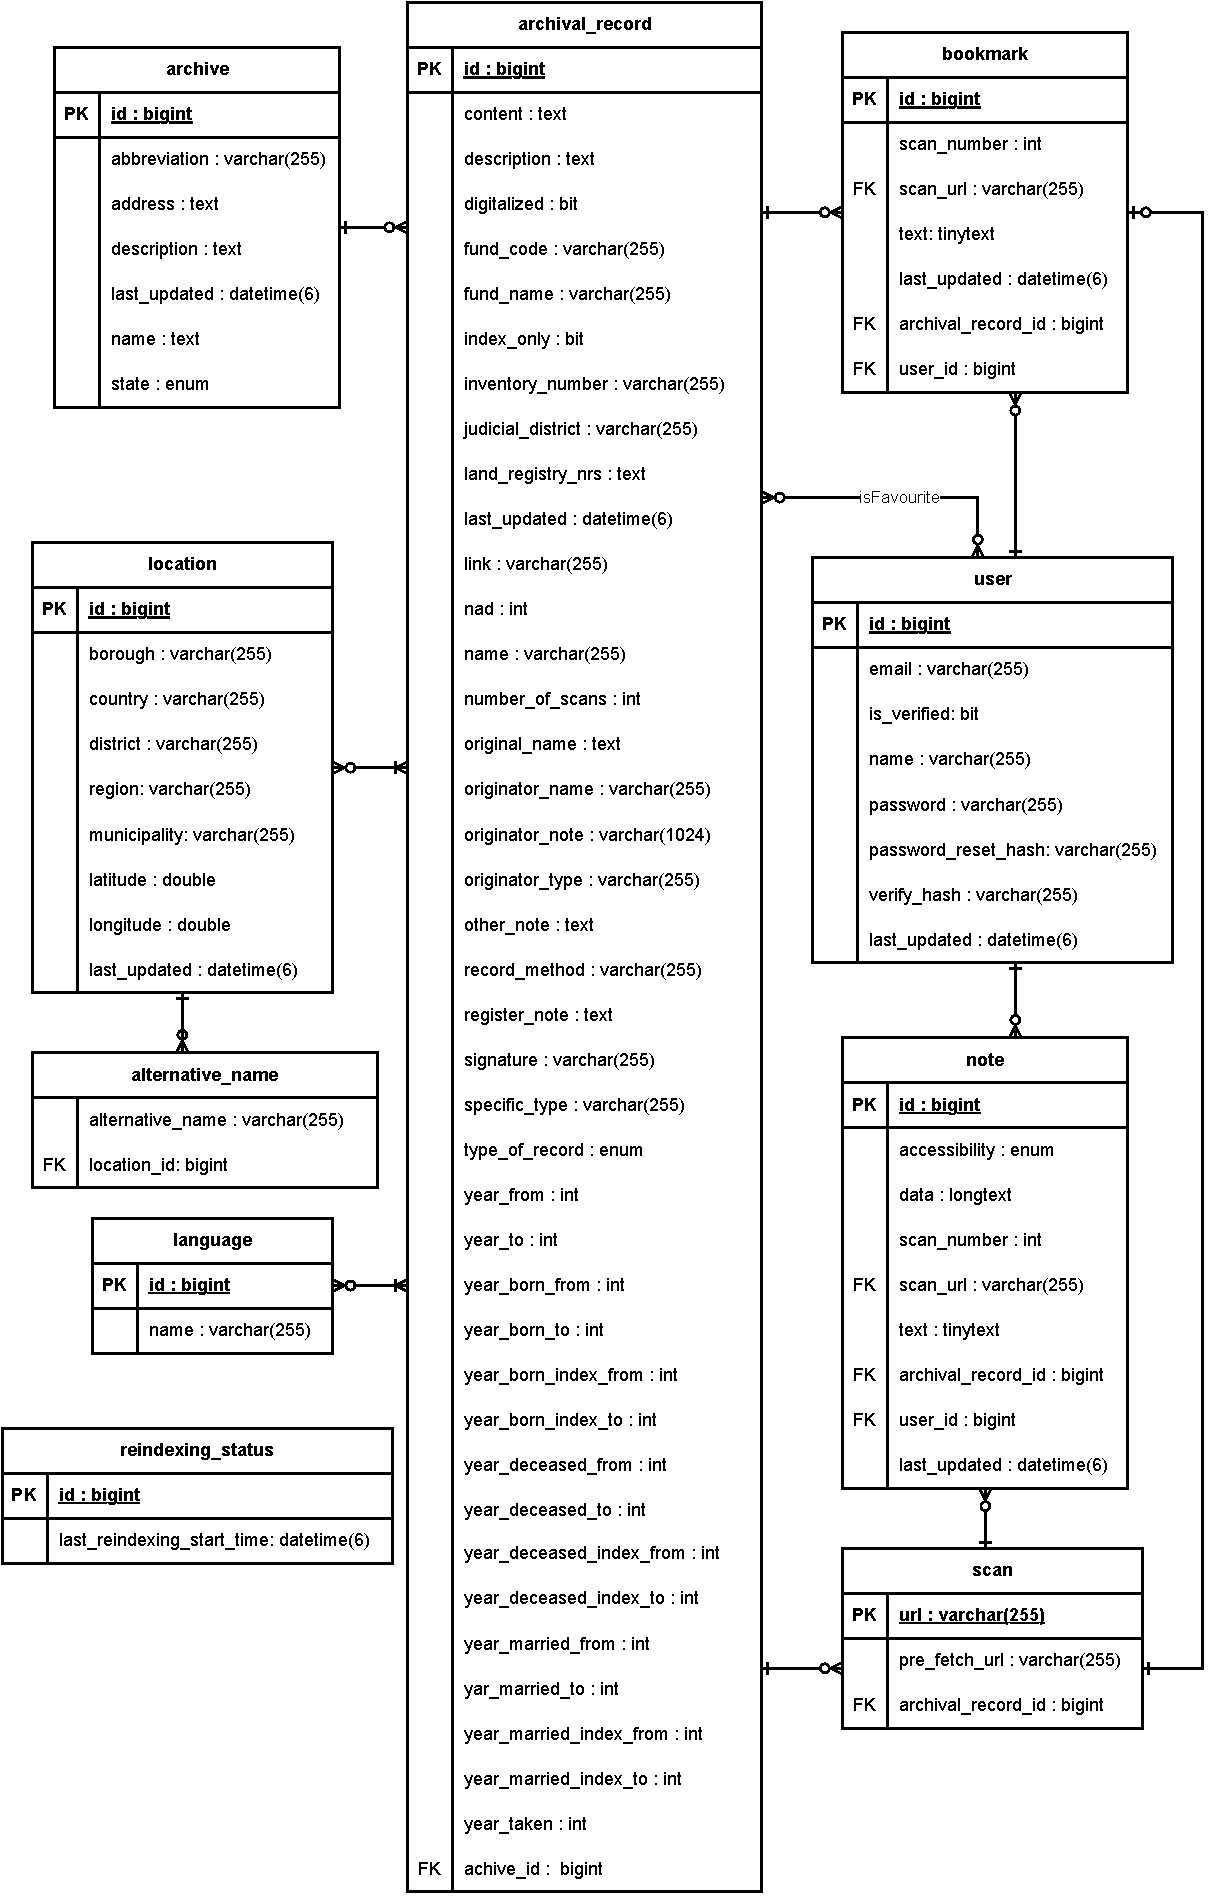
\includegraphics[scale=.7]{obrazky-figures/design/er_diagram.pdf}
        \caption{Entity-relationship diagram}
\end{figure}


\newpage
\section{Diagramy struktury}
Strukturální UML diagramy pomáhají popsat architekturu aplikace na úrovni jednotlivých subsystémů, komponent a balíků. Oproti předchozím diagramům se již nezaměřují na popsání požadavků na nově vznikající systém, ale návrhář je využije při tvorbě návrhu architektury aplikace. Jedná se o velmi vhodné dokumentační diagramy, které usnadní pochopení vazeb mezi jednotlivými částmi systému bez nutnosti nahlížení do zdrojového kódu.

\subsection{Vysokoúrovňový diagram komponent}
Úlohou diagramu komponent \cite{componentDiagram} na nejvyšší úrovni je rozdělení řešeného problému do jednotlivých služeb, které spolu budou kooperovat. V rámci této práce bude systém rozdělen do čtyř služeb, dvou databází a jedné externí služby pro odesílání e-mailových zpráv. Klasická architektura klient-server je rozšířena o~další služby, jež se starají o stahování dat ze všech archivů a přístup k~mediálním datům jednotlivých archiválií.

\begin{figure}[htbp]
\centering
    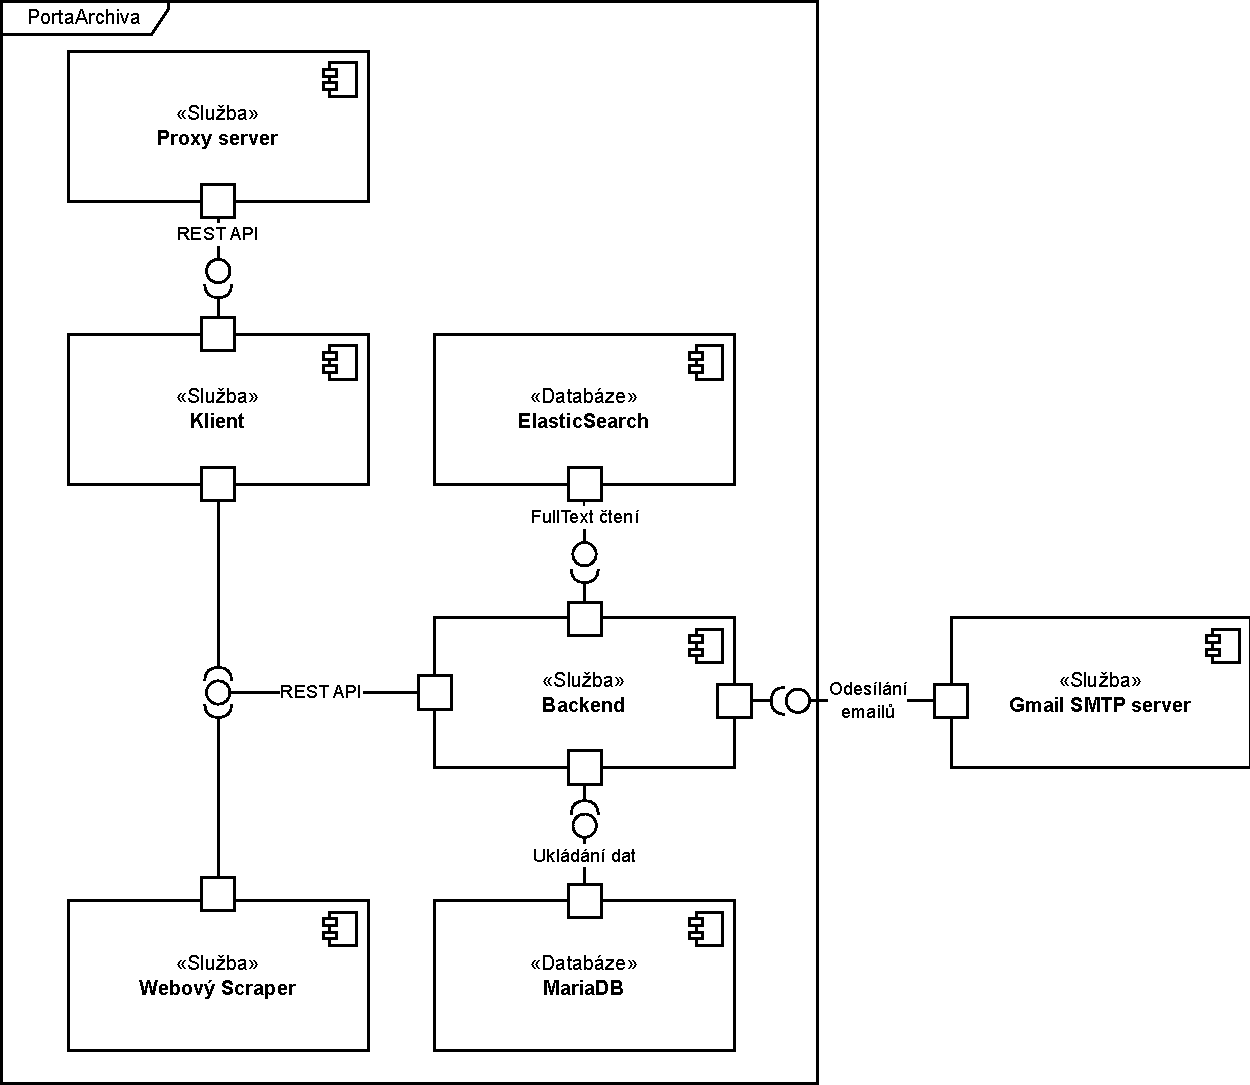
\includegraphics[scale=.72]{obrazky-figures/design/high_level_component_diagram.pdf}
    \caption{Vysokoúrovňový diagram komponent}
\end{figure}

\newpage
\subsection{Diagram komponent Webového scraperu} 
Úlohou Webového scraperu je stahování dat z webových stránek jednotlivých archivů. Systém používá aplikační rámec Scrapy a~je napsán v~Pythonu. Autorem systému je Jan Valušek \cite{Valusek}, ovšem pro potřeby tohoto projektu bylo nutné stávající řešení adaptovat. Tento systém je vybrán z~jednotlivých systémů na základě provedených kontrol konzistence datových sad a díky podpoře pro stahování mediálních dat jednotlivých archiválií. Jádrem aplikace jsou scripty pro jednotlivé archivy ve složce \texttt{Spiders}, které používají pomocné moduly jako \texttt{Auxiliary} a \texttt{Constants}. Moduly \texttt{Middlewares}, \texttt{Items}, \texttt{Settings} a \texttt{Pipelines} se věnují nastavení prostředí pro aplikační rámec Scrapy, zpracování záznamu a odeslání přes API na serverovou část aplikace. \texttt{LocationModule} se používá k vyhledávání jednotlivých lokalit pomocí API \href{https://www.openstreetmap.org/}{OpenStreetMap}. 
\texttt{LocationModule} pro každou hledanou lokalitu vrátí více možných výsledků a je tedy úlohou \texttt{ClusteringModule} vybrat tu nejpravděpodobnější správnou lokalitu. Princip algoritmu bude blíže popsán v kapitole \ref{chap:implementation} Implementace.

\begin{figure}[htbp]
\centering
    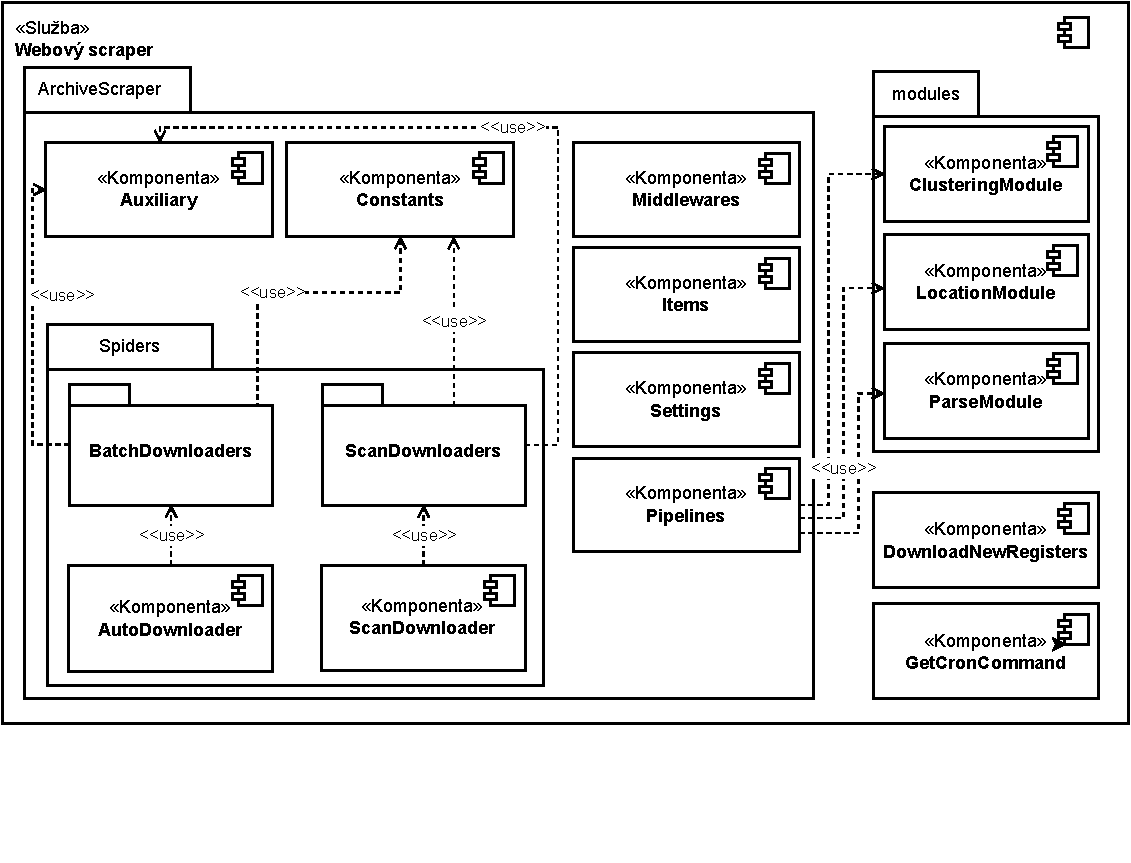
\includegraphics[scale=.76]{obrazky-figures/design/scraper_component_diagram.pdf}
    \caption{Diagram komponent webového scraperu}
\end{figure}

\subsection{Diagram komponent klientské aplikace}
Jelikož se jedná se webovou aplikaci, tak i~zde existuje startovní bod \texttt{Index}, v rámci kterého se volá \texttt{router}. \texttt{Router} se stará o~mapování URL adresy na příslušné \texttt{view}. \texttt{Router} dále řeší zvolený \texttt{layout} aplikace, jenž se může lišit například na základě toho, zda je uživatel přihlášen. \texttt{View} reprezentuje jednu stránku naší aplikace jako například úvodní stránku, seznam archiválií, detail archiválie a~další. Každý tento \texttt{view} se skládá z~jednotlivých \texttt{komponent}. \texttt{Komponenta} je znovupoužitelný kus kódu. Rozdělení systému do jednotlivých \texttt{komponent} umožňuje udržovat velikost jednotlivých zdrojových souborů v~rozumném rozsahu, což zjednodušuje případné rozšíření a~údržbu aplikace. Každá komponenta může mít svůj interní stav a~pomocné funkce, které například reagují na specifickou událost. Hlavním úkolem komponenty je vykreslit část výsledného \texttt{view} a~přidáním pomocných funkcí nebo stavových proměnných by byl porušen princip jedné zodpovědnosti. K tomu, aby došlo k oddělení komponenty od logiky, je nutné pomocné funkce (stavové proměnné a~event handlery) vytknout do separátního \texttt{hooku}, jenž je následně využit v~komponentě. Problém nastává při použití \texttt{hooku} ve více komponentách, kdy je nutné mezi nimi sdílet stav \texttt{hooku}. Sdílení stavu mezi komponentami lze dosáhnout pomocí \texttt{kontextu} umožňujícího sdílet stavové proměnné jednoho \texttt{hooku}. Ke každé komponentě se vztahuje její \texttt{Styles} modul, který obsahuje definici stylů pro konkrétní komponentu. Použití modulů způsobí, že za název použité \texttt{scss} třídy se vygeneruje hash, takže v~případě, kdy je použit stejný název třídy ve dvou komponentech, nedojde ke kolizi těchto stylů. \texttt{Komponenta} kromě stavových proměnných potřebuje přístup ke statickým souborům, jež jsou uloženy v modulu \texttt{assets}. Další pomocné funkce jsou zabalené v modulu \texttt{utils} a v případě formulářů v~modulu \texttt{validators}. Doposud byla rozebrána pouze problematika tvorby komponent, validace a~zobrazení \texttt{view}. To, co doposud chybělo, byla komunikace s~API. Pro uchovávání dat na klientovi je využita knihovna \texttt{Redux} sloužící jako centralizované úložiště, a~její detailní popis je uveden v kapitole \ref{chap:implementation} Implementace. Pokud posílá komponenta požadavek na API, tak používá \texttt{ActionHook} a~pro přístup ke staženým datům používá \texttt{SelectorHook}, kde jsou data neměnná. Na první pohled se může jednat o zbytečnou režii a nabízí se otázka, proč nelze rovnou upravovat a~číst data z jedné proměnné jako například v~aplikačním rámci \texttt{Vue.JS}. V~rámci malých projektů se vskutku jedná o~zbytečnou režii, ale na větších projektech to pomáhá držet čistou architekturu a~vzniká méně chyb v~kódu, jelikož se striktně rozlišuje, kdy může být hodnota čtena a~kdy modifikována.
\begin{landscape}
    \begin{figure}[htbp]
    \centering
        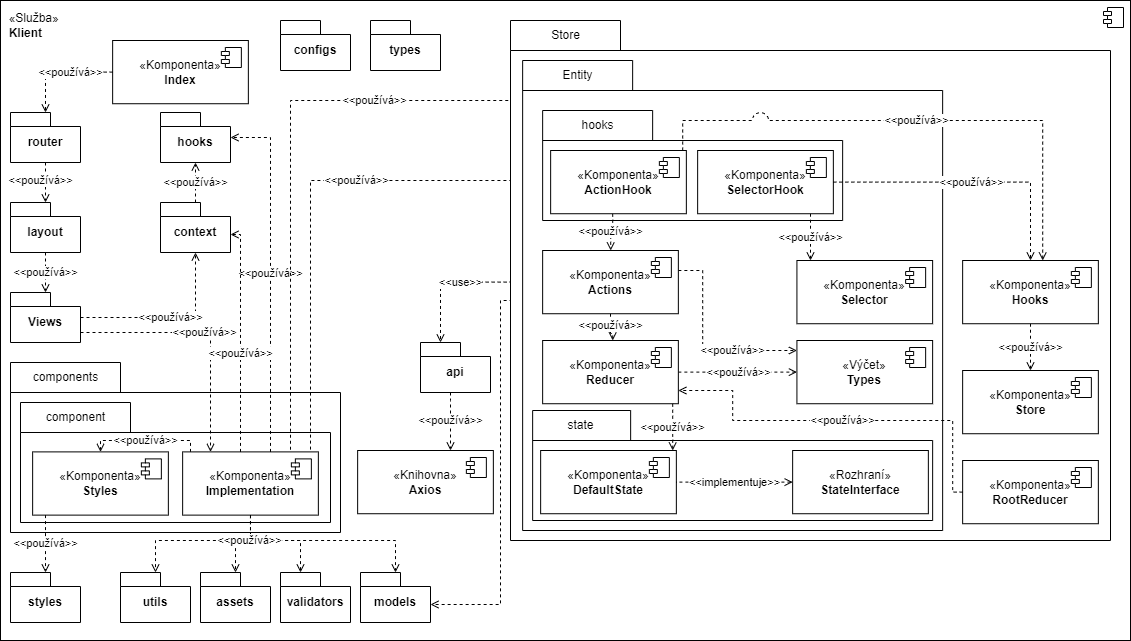
\includegraphics[scale=.6]{obrazky-figures/design/client_component_diagram.png}
        \caption{Diagram komponent klienta}
    \end{figure}
\end{landscape}

\subsection{Diagram komponent serverové části aplikace}
Serverová část je standardní monolitická aplikace, kde je vhodné použít třívrstvou architekturu. Spodní vrstva je technického charakteru a převážně zodpovídá za připojení k~datovým úložištím. Nad datovou vrstvou je aplikační logika, která je vždy závislá na konkrétní aplikaci, jelikož implementuje jednotlivé případy užití. Třetí vrstva zajišťuje, aby operace, které jsou definované v~aplikační logice, byly poskytnuty ostatním službám přes aplikační rozhraní. V~tomto případě bylo zvoleno konzervativní rozhraní REST. 
\newpara
Modul \texttt{core} obsahuje podpůrné nastavení. Modul \texttt{commandLineRunners} obsahuje funkce, jež se spouští při startu aplikace. Je zde například umístěna inicializace databáze. Dále je zde definice typů pro databázi ElasticSearch, nastavení pro JSON Web Token a definice jednotlivých výjimek, které aplikace vyvolává v případě chyby. 
\newpara
Nejnižší vrstva zodpovídá za přístup k~databázím, definici entit a~jedná se o~základní stavební kámen serverové aplikace. V~tomto případě se jedná o~balík \texttt{domain}. V~rámci balíku \texttt{domain} jsou definovány entity, jež vzhledem k~návrhu ER diagramu vyžadují pomocné \texttt{embeddable} a~\texttt{enums}. Vzhledem k~tomu, že je použita jedna entita pro relační i~nerelační databázi, tak pro použití Elasticsearch je potřeba definovat vlastní převodníky pro převod konkrétního datového typu do databáze a zpět. Tyto převodníky jsou definovány v balíku \texttt{converters} a \texttt{bridges}. Použití \texttt{Java persistence API} umožňuje definici repozitářů pouze pomocí rozhraní bez nutnosti implementovat veškeré základní operace jako například získání záznamu podle identifikátoru. Ne vždy nám bohužel stačí tato základní sada, která lze pomocí \texttt{Java persistence API} vygenerovat, a proto jsou tyto základní \texttt{repozitáře} zapouzdřeny do \texttt{persistenceService}. V rámci \texttt{persistenceService} jsou implementovány všechny chybějící dotazy na databázi. Pomocné znovupoužitelné predikáty jsou definovány v rámci modulu \texttt{specs}.
\newpara
Separátní \texttt{persistenceService} a \texttt{specs} umožňují držet čitelnou aplikační logiku implementovanou v balíku \texttt{service}. Struktura entity musí odpovídat struktuře tabulky v databázi. Pokud operace nemá vracet všechna data z databáze, tak se využije \texttt{mapper}, jenž dokáže mapovat objekty různých datových typů. Vhodným mapováním se šetří čas, který by byl nutný pro přenos nepotřebných atributů skrze protokol HTTP na klienta. Pro mapování existuje více alternativních knihoven, jež se dělí podle toho, jak provádí mapování. Některé knihovny využívají reflexi, což je mocný nástroj interpretovaných jazyků, který je ovšem velmi nákladný na výpočetní zdroje. Reflexe umožňuje za běhu analyzovat a měnit strukturu chování, takže lze získat informace o třídách, metodách a polích, a také je volat a manipulovat s nimi, aniž by bylo nutné znát tyto detaily předem při kompilaci kódu. Alternativní přístup k mapování je analýza v době překladu, kde jsou jednotlivé třídy zodpovědné za mapování vygenerovány staticky a není tak nutné provádět analýzu za běhu.
\newpara
V rámci nejvyšší vrstvy je řešeno poskytování aplikační logiky a interakce s okolím. Jelikož bylo zvoleno rozhraní REST, tak \texttt{controllery} obsahují definici jednotlivých koncových bodů, přes které může uživatel volat jednotlivé operace byznys logiky.
\newpara
Pro definici aplikačního rozhraní dané aplikace byl zvolen dokumentační standard OpenAPI, jenž striktně definuje, jak popsat rozhraní aplikace, a to včetně typů parametrů, návratových hodnot a popisu jednotlivých koncových bodů. Popis je uložen v samostatném projektu OpenApiSpec a pro každý \texttt{controller} existuje separátní \texttt{YAML} soubor. Tuto specifikaci je možno importovat do nástroje Postman nebo ji interaktivně procházet pomocí nástroje Swagger.


\begin{figure}[htbp]
    \centering
    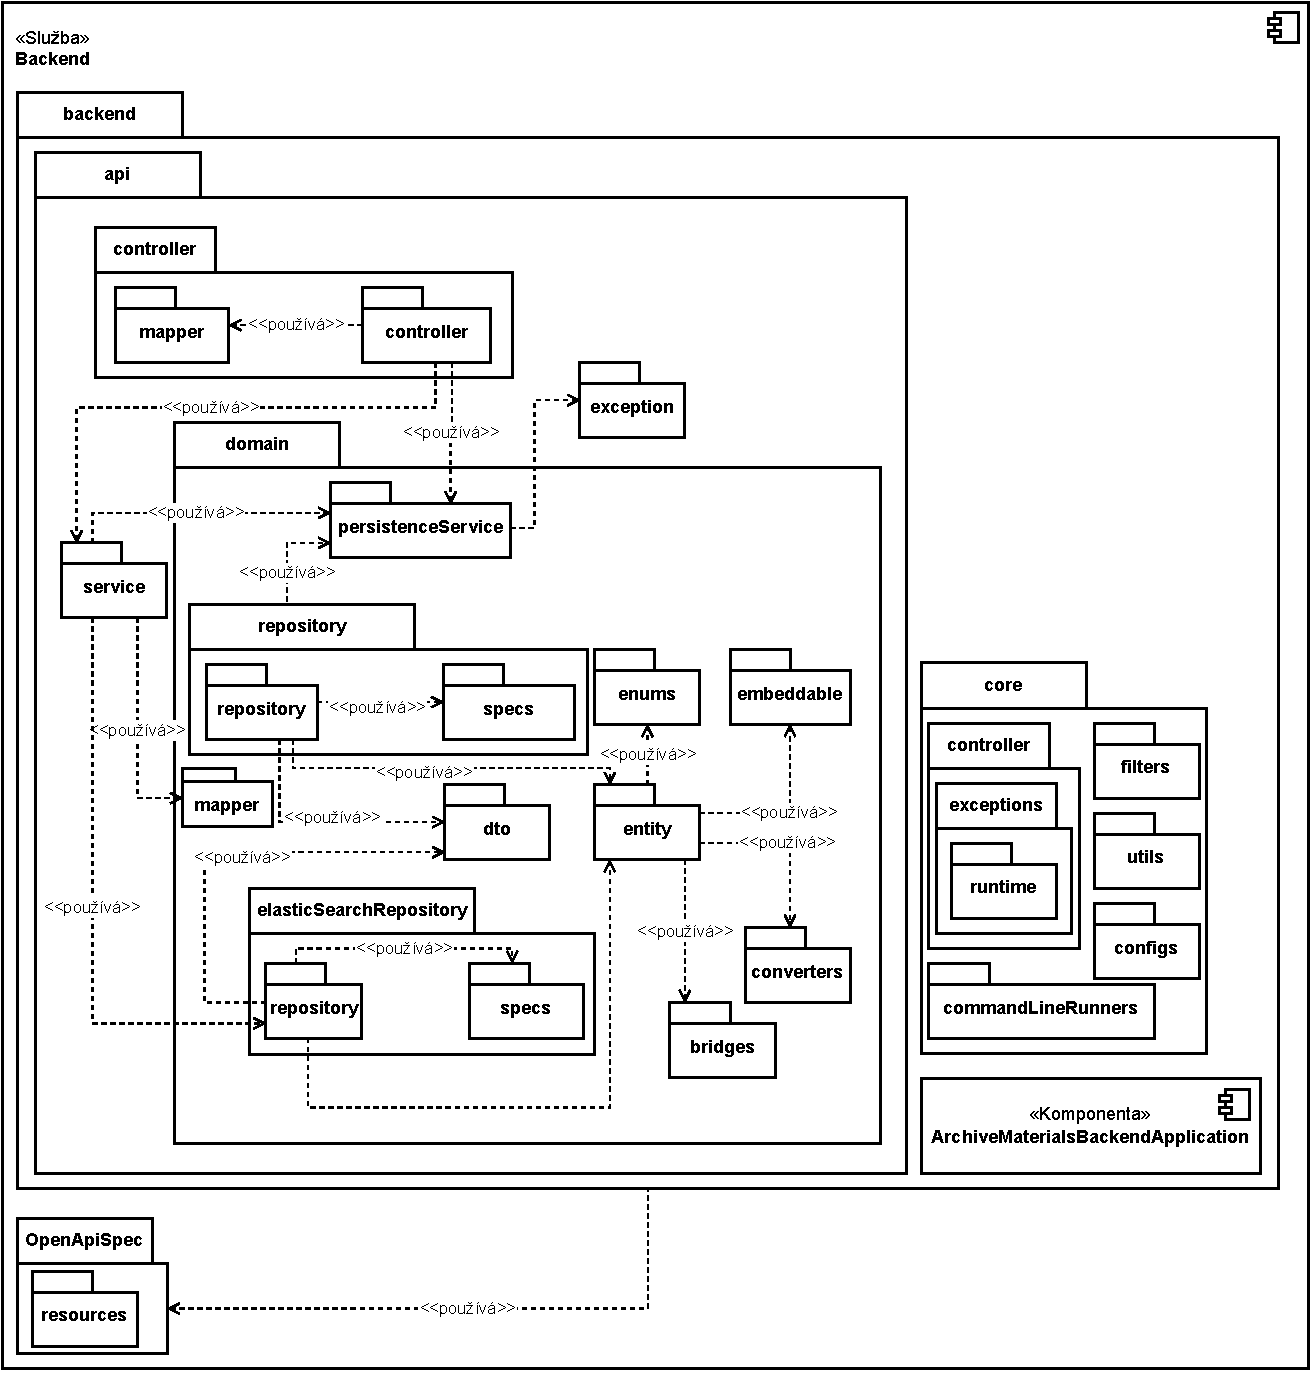
\includegraphics[scale=.65]{obrazky-figures/design/backend_component_diagram.pdf}
    \caption{Diagram komponent serverové části aplikace}
\end{figure}



%\section{Tvorba dotazníku na prototyp}

%\section{Zhodnocení dotazníku}

\newpage
\section{Tvorba konečného automatu přechodů}
\label{sec:transitionStateMachine}
Diagram reprezentuje jednotlivé pohledy v~rámci systému jako stavy. Hrany značí možný přechod mezi pohledy. Z~každého pohledu se lze implicitně přesunout na hlavní stránku, a~to pomocí navigačního menu.
\begin{figure}[htbp]
\centering
    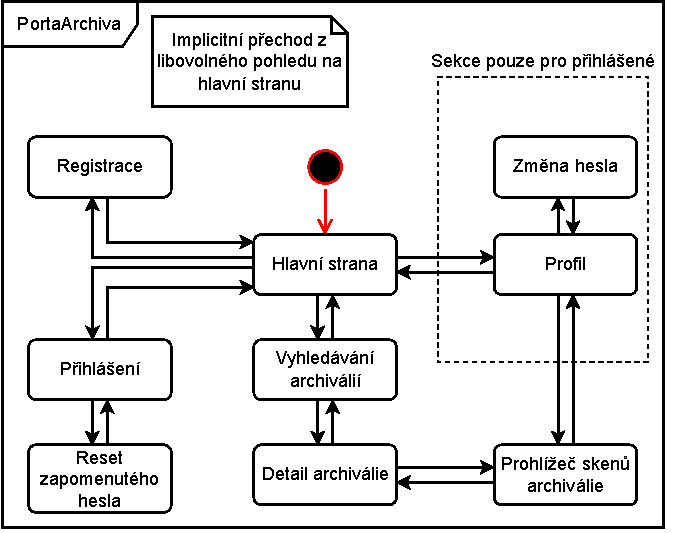
\includegraphics[scale=1.2]{obrazky-figures/design/PageTransitionStateMachine.pdf}
    \caption{Konečný automat přechodů}
\end{figure}

\newpage
\section{Tvorba grafického návrhu}
Pro tvorbu grafického návrhu byl zvolen nástroj \href{https://www.figma.com}{Figma} \cite{figma}. Jedná se o~online kolaborativní nástroj pro tvorbu interaktivních prototypů. Nejedná se tedy o~pouhé obrázky, ale uživatel může s~prototypem interagovat a~navigovat se napříč pohledy. Díky možnosti tvorby vlastních komponent urychluje jak samotnou tvorbu prototypu, tak i~následně úpravu podle představ zadavatele. Do Figmy lze doinstalovat mnoho přídavných balíků, a to například pro kontrolu kontrastu jednotlivých komponent nebo sadu ikon.
\newpara
Interaktivní prototyp\footnotemark se skládá z~jednotlivých pohledů a~různých překryvných prvků aplikujících se při spuštění určité události nad konkrétním prvkem. Dále jsou zde definovány přechody mezi pohledy, které byly navrženy při tvorbě konečného automatu přechodů v kapitole ~\ref{sec:transitionStateMachine} Tvorba konečného automatu přechodů. Výsledný návrh vznikal iterativně a~vždy byl konzultován s~vedoucím práce, jenž sdělil konstruktivní kritiku a~náměty na změny. V~následujícím textu jsou uvedeny ukázky pohledů z~návrhu, a~to včetně popisu rozložení.

\footnotetext{\href{https://www.figma.com/proto/90Nm3ZEx48DYMICGL7u0MP/Master-Thesis?node-id=281-4650&t=cITZe8WZ8ckybige-1}{https://www.figma.com/proto/90Nm3ZEx48DYMICGL7u0MP/Master-Thesis?node-id=281-4650\&t=cITZe8WZ8ckybige-1}}

\begin{figure}[htbp]
\centering
    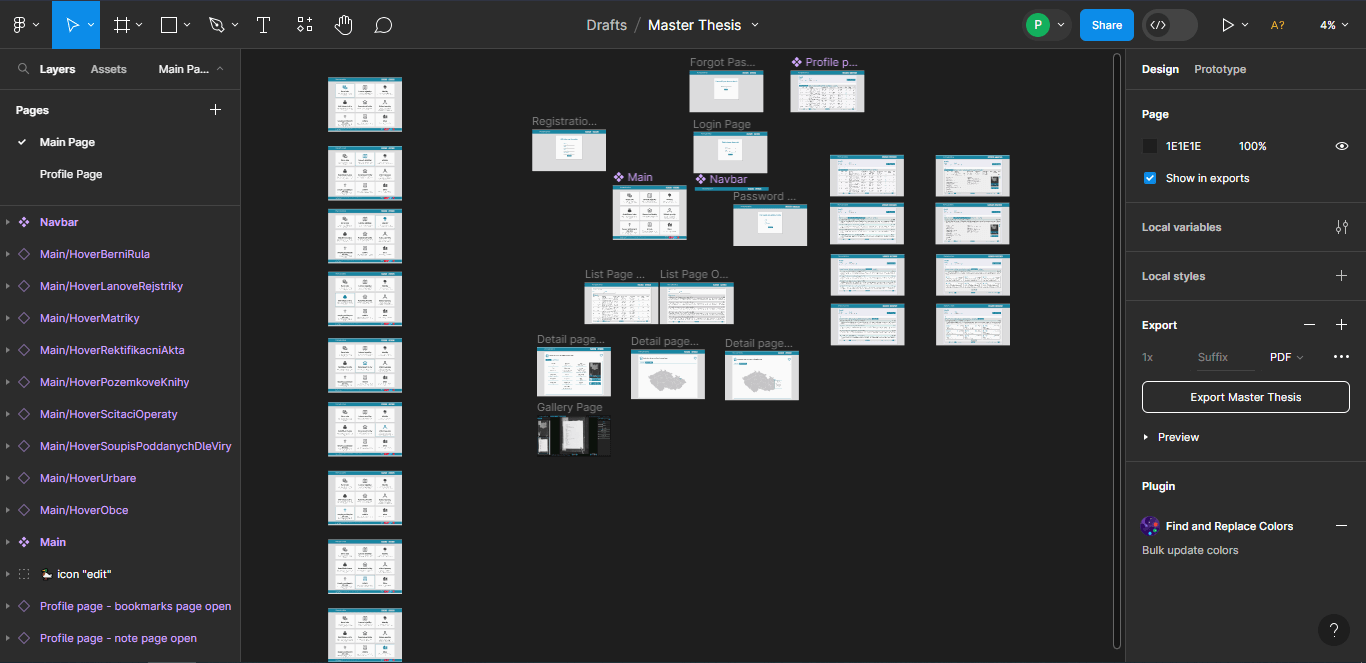
\includegraphics[scale=.3]{obrazky-figures/design/figma/project_overview.png}
    \caption{Návrhový režim ve Figmě}
\end{figure}
\noindent
Při návrhu titulní strany byl kladen důraz na tvorbu rychlého rozcestníku pro uživatele, kde by si uživatel zvolil, v~rámci jakých pramenů chce hledat, případně zda chce vyhledávat podle lokality. Každá kategorie je doplněna krátkým popisem sloužícím k~rychlejší orientaci začínajícímu badateli.

\begin{figure}[htbp]
\centering
    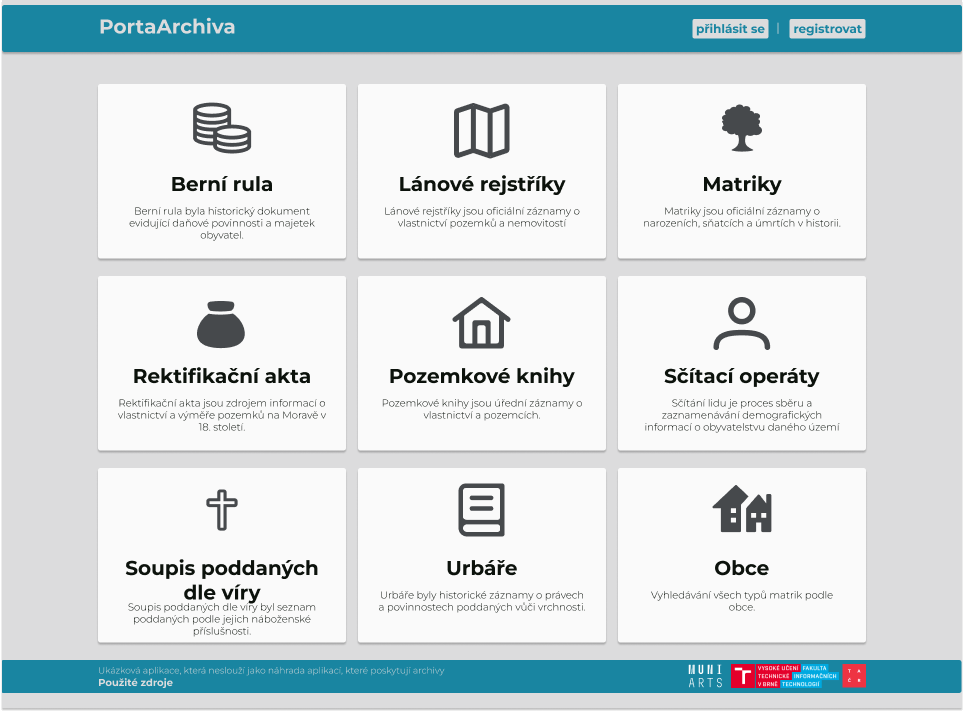
\includegraphics[scale=.4]{obrazky-figures/design/figma/Main.png}
    \caption{Návrh titulní strany ve Figmě}
\end{figure}

\newpage
\noindent
Seznam archiválií obsahuje plné textové vyhledávání i~specifické vyhledání některých atributů v~horní části pohledu. Seznam záznamů má formu tabulky, kde ovládání je umístěno v~jejím záhlaví. Po kliknutí na záznam je uživatel přesměrován na detail daného záznamu. Na základě konzultace s~vedoucím práce byl použit podobný formát z~již existujících řešení, a to z toho důvodu, aby se usnadnil přechod badatelům z dosavadních systémů.
\newpara
Seznam matrik obsahuje základní informace, kde odznak u obcí značí počet obcí v~dané archiválii a~po najetí kurzoru na odznak se zobrazí podrobný seznam obcí.

\begin{figure}[htbp]
\centering
    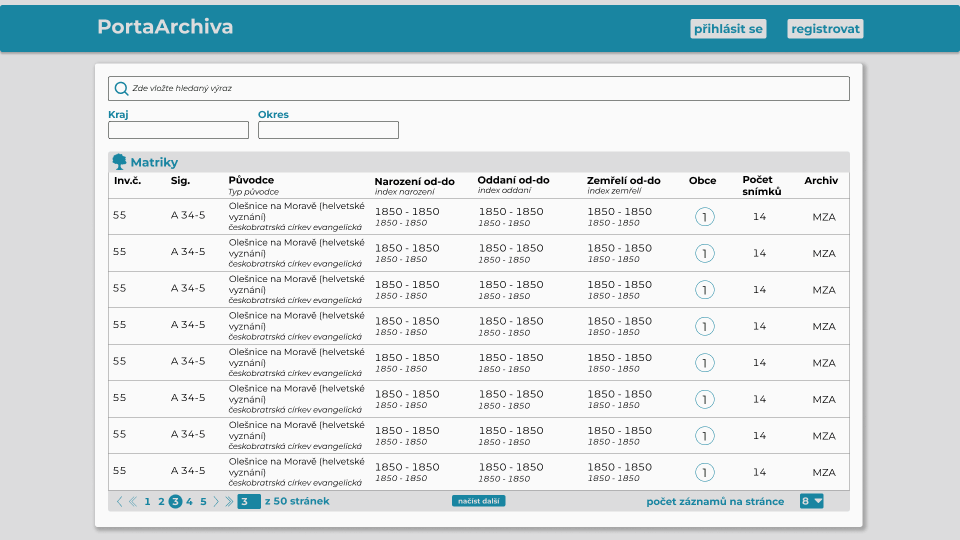
\includegraphics[scale=.4]{obrazky-figures/design/figma/List Page Matriky.png}
    \caption{Seznam matrik}
\end{figure}

\newpage
\noindent
Pro ostatní typy archiválií byl zvolen odlišný formát vizualizace záznamu tabulky, jelikož matriky obsahují specifické informace, které ostatní typy archiválií neobsahují.

\begin{figure}[htbp]
\centering
    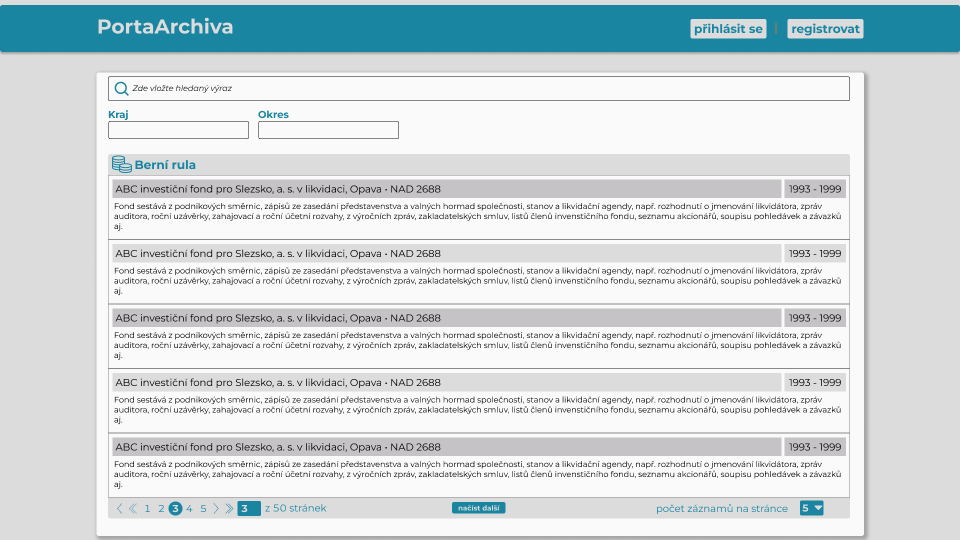
\includegraphics[scale=.4]{obrazky-figures/design/figma/List Page Ostatni.png}
    \caption{Seznam archiválií pro ostatní typy archiválií}
\end{figure}
\noindent
Po zvolení záznamu ze seznamu archiválií se zobrazí podrobnější informace o dané archiválii a~v záložce územní rozsah si uživatel interaktivně zobrazí území na mapě, odkud daná archiválie pochází. Uživatel může dále zobrazit digitalizované snímky archiválie, případně přejít na detail archiválie na stránkách archivu, odkud daný záznam pochází. Uživatel má možnost si uložit archiválii do oblíbených v~případě, že je v~systému přihlášený.

\begin{figure}[htbp]
\centering
    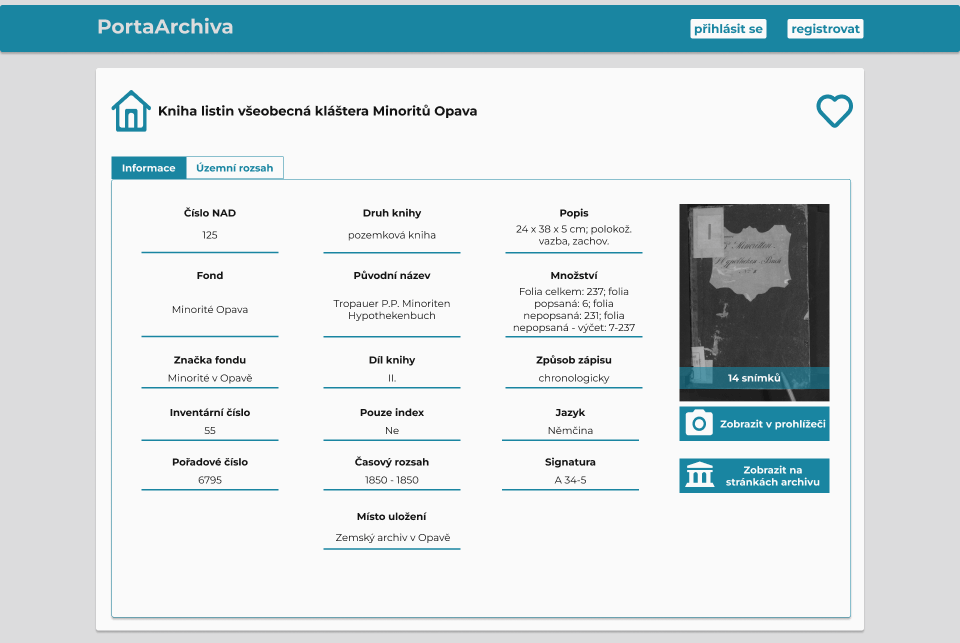
\includegraphics[scale=.4]{obrazky-figures/design/figma/Detail page - info.png}
    \caption{Detailní pohled na archiválii}
\end{figure}

\newpage
\noindent
V případě, že je uživatel přihlášený, tak má přístup ke svému profilu. V profilu aplikace může kromě změny osobních a~přihlašovacích údajů také spravovat svoje oblíbené archiválie, přidané záložky a~osobní poznámky v~rámci systému.

\begin{figure}[htbp]
\centering
    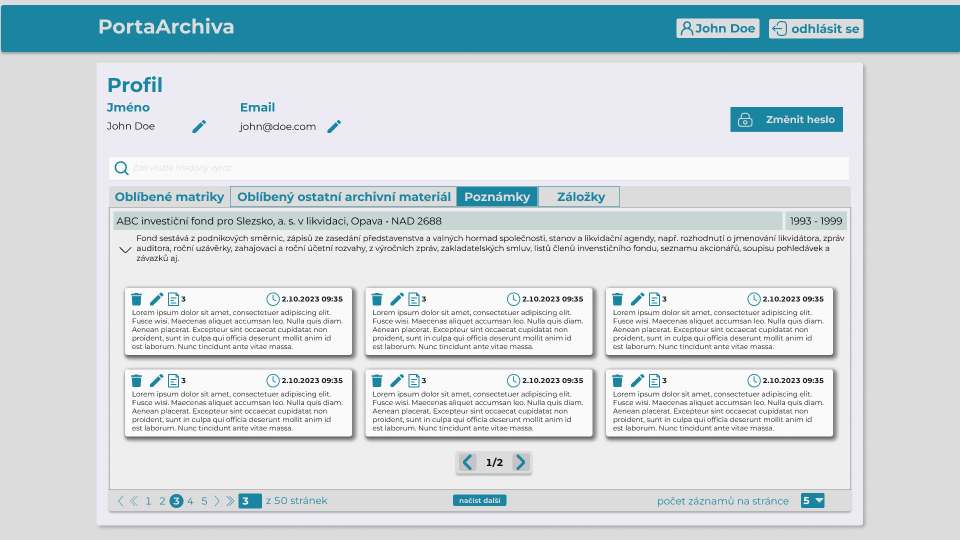
\includegraphics[scale=.4]{obrazky-figures/design/figma/Profile page - note page open.png}
    \caption{Detailní pohled na archiválii}
\end{figure}
\newpage
Samotné jádro aplikace je prohlížeč digitalizovaných snímků archiválií, který vychází z~rozložení použitého při tvorbě interaktivního prototypu, jenž byl představen v kapitole \ref{sec:funkcni-prototyp} Tvorba interaktivního prototypu. Hlavní ovládací panel se nachází v~horní části obrazovky a je doplněn o základní informace aktuálně prohlížené archiválie. 

\begin{figure}[htbp]
\centering
    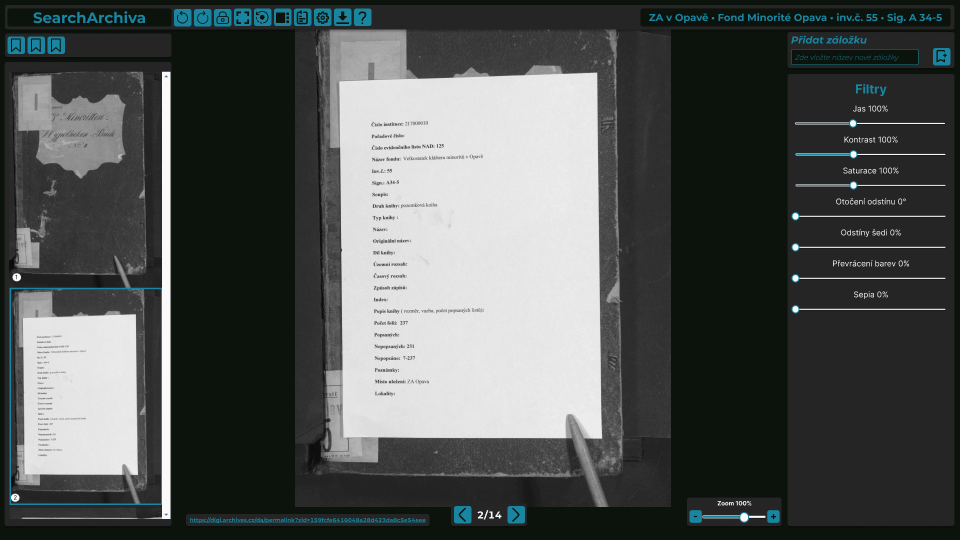
\includegraphics[scale=.4]{obrazky-figures/design/figma/Gallery Page.png}
    \caption{Prohlížeč snímků archiválie}
\end{figure}




